\documentclass[12pt, titlepage]{article}
\usepackage[utf8]{inputenc}
\usepackage[T1]{fontenc}
\usepackage[a4paper, margin=0.7in]{geometry}
\usepackage{amsfonts}
\usepackage{mathabx}
\usepackage{listings}
\usepackage{xcolor}
\usepackage{subcaption}
\usepackage{multirow}
\usepackage{makecell}
\usepackage{pgfplots}

\usepackage{minted}
\documentclass[border=2mm]{standalone}
\usemintedstyle{perldoc}

\usepackage{hyperref}
\definecolor{blackgray}{rgb}{0.22,0.22,0.26}
\definecolor{whiteish}{rgb}{0.97, 0.97, 0.96}
\definecolor{greener}{rgb}{0.961, 0.941, 0.902}
\definecolor{greenish}{rgb}{0.35, 0.51, 0.34}

\pagecolor{whiteish}

\title{IT45: TP3}

\author{Yann Derré}
\date{April 2023}
\hypersetup{
  colorlinks=true,
  linkcolor=greenish,
  urlcolor=greenish,
}

\begin{document}
\color{blackgray}
\maketitle

\begin{abstract}

Le code est exécuté sur un processeur M1 et compilé avec le flag \texttt{-O3} pour bénéficier de l'accélération matérielle de la vectorisation des calculs. Code source est disponible sur mon \href{https://github.com/derreyann/}{Repo GitHub}.

\tableofcontents

\end{abstract}

\newpage

\section{Travail préparatoire}
\subsection{Calcul des distances}

Pour utiliser l'algorithme de Little, nous calculons la matrice de distances entre une ville A et B. Nous utilisons la formule de la distance entre 2 points dans une space cartésien à 2 dimensions.
\[
  \quad D_{ij} = \sqrt{(x_i - x_j)^2 + (y_i - y_j)^2} avec \forall i \neq j
\]

Voici la fonction en C:

\begin{minted}
[
fontsize=12
baselinestretch=1.2,
fontsize=\footnotesize,
linenos,
bgcolor=greener
]
{C}
void compute_dist_matrix()
{
    for (int i = 0; i < NBR_TOWNS; i++)
    {
        int j = 0;
        while (j < i)
        {
            dist[i][j] = sqrt(pow(coord[i][0] - coord[j][0], 2) 
            + pow(coord[i][1] - coord[j][1], 2));
            dist[j][i] = dist[i][j];
            j++;
        }
        dist[i][i] = -1;
    }
}
\end{minted}

A la ligne 12, nous appliquons dans la matrice de la distance une restriction du trajet la ville sur elle-même en lui donnant la valeur -1. 

\subsection{Création de l'heuristique "nearest neighbour"}

Pour faire fonctionner l'algorithme de Little, nous utilisons comme heuristique la borne initiale de la distance parcourue pour ignorer les branches non optimales. Cela nous donne également une approximation de la solution optimale.


\begin{minted}
[
fontsize=12
baselinestretch=1.2,
fontsize=\footnotesize,
linenos,
bgcolor=greener
]
{C}
double build_nearest_neighbour()
{
    /* solution of the nearest neighbour */
    int i, sol[NBR_TOWNS];

    /* evaluation of the solution */
    double eval = 0;

    // On initialise les villes à 0
    for (i = 0; i < NBR_TOWNS; i++)
    {
        sol[i] = 0;
    }

    //Trouve la ville la plus proche de la ville actuelle
    for (i = 1; i < NBR_TOWNS; i++)
    {
        double min = -1;
        int k;
        for (int j = 0; j < NBR_TOWNS; j++)
        {
            for (k = 0; k < i; k++)
            {
                if (sol[k] == j)
                {
                    break;
                }
            }
            if (k < i)
            {
                //La ville est déjà visitée?
                continue;
            }
            if (min < 0 || dist[sol[i - 1]][j] < min)
            {
                //Ville actuelle plus intéressante
                min = dist[sol[i - 1]][j];
                sol[i] = j;
            }
        }
    }

    eval = evaluation_solution(sol);
    printf("Nearest neighbour ");
    print_solution(sol, eval);

    for (i = 0; i < NBR_TOWNS; i++)
        best_solution[i] = sol[i];
    best_eval = eval;

    return eval;
}


\end{minted}
\section{Algorithme de Little}

\subsection{Setup matrice des distances}

On fait apparaître un zéro dans chaque colonne de la matrice des distances en effectuant la soustraction avec le minimum de chaque colonne.

\begin{minted}
[
fontsize=12
baselinestretch=1.2,
fontsize=\footnotesize,
linenos,
bgcolor=greener
]
{C}
    for (i = 0; i < NBR_TOWNS; i++)
    {
        double min = INFINITY;
        for (j = 0; j < NBR_TOWNS; j++)
        {
            if (d[i][j] < min)
            {
                if (d[i][j] != -1)
                    min = d[i][j];
            }
        }
        for (j = 0; j < NBR_TOWNS; j++)
        {
            if (d[i][j] != -1)
                d[i][j] -= min;
        }
        if (min != INFINITY)
            eval_node_child += min;
    }

    // Check if 0 in every column

    for (j = 0; j < NBR_TOWNS; j++)
    {
        double min = INFINITY;
        for (i = 0; i < NBR_TOWNS; i++)
        {
            if (d[i][j] < min)
            {
                if (d[i][j] != -1)
                    min = d[i][j];
            }
        }
        for (i = 0; i < NBR_TOWNS; i++)
        {
            if (d[i][j] != -1)
                d[i][j] -= min;
        }
        if (min != INFINITY)
            eval_node_child += min;
    }
\end{minted}

La distance -1 est également ignorée pour ne pas explorer les villes marquées dans la création de la matrice des distances. On vérifie que la nouvelle valeur trouvée par eval ne dépasse pas la meilleure trouvée, en stoppant la recherche du node si le check ne passe pas


\begin{minted}
[
fontsize=12
baselinestretch=1.2,
fontsize=\footnotesize,
linenos,
bgcolor=greener
]
{C}
    /* Cut : stop the exploration of this node */
    if (best_eval >= 0 && eval_node_child >= best_eval)
        return;
\end{minted}

\subsection{Identifier les pénalités}

On identifie le zéro avec la plus grosse pénalité, c'est-à-dire la somme des plus petites valeurs de la ligne et de la colonne 0. On itère sur chaque 0 en comparant avec la pénalité précédente, en fixant une pénalité infinie sur les 0 déjà explorés et mémorisant la pénalité la plus grande.


\begin{minted}
[
fontsize=12
baselinestretch=1.2,
fontsize=\footnotesize,
linenos,
bgcolor=greener
]
{C}
    int izero = -1, jzero = -1;
    double max_penalty = -1;
    for (i = 0; i < NBR_TOWNS; i++)
    {
        for (j = 0; j < NBR_TOWNS; j++)
        {
            if (d[i][j] == 0)
            {
                double penalty_x = INFINITY, penalty_y = INFINITY;
                double visited_x = 0, visited_y = 0;
                for (int k = 0; k < NBR_TOWNS; k++)
                {
                    if (k != i && d[k][j] < penalty_x && d[k][j] >= 0)
                    {
                        penalty_x = d[k][j];
                        visited_x = 1;
                    }
                    if (k != j && d[i][k] < penalty_y && d[i][k] >= 0)
                    {
                        penalty_y = d[i][k];
                        visited_y = 1;
                    }
                }
                double penalty = penalty_x + penalty_y;
                if (penalty > max_penalty && (visited_x || visited_y))
                {
                    max_penalty = penalty;
                    izero = i;
                    jzero = j;
                }
                else if (visited_x == 0 && visited_y == 0)
                {
                    max_penalty = INFINITY;
                    izero = i;
                    jzero = j;
                }
            }
        }
    }

//Si on ne trouve pas de 0, sortie !! Pour plus tard, l'élimination des sous-tours peut avoir supprimé les solutions possibles.
    if (izero == -1 || jzero == -1)
    {
        return;
    }
//Mise à jour de la solution avec notre 0 choisi.
    starting_town[iteration] = izero;
    ending_town[iteration] = jzero;

        /* Do the modification on a copy of the distance matrix */
    double d2[NBR_TOWNS][NBR_TOWNS];
    memcpy(d2, d, NBR_TOWNS * NBR_TOWNS * sizeof(double));

    /* Modify the dist matrix to explore the choice of the zero with the max penalty */
    for (i = 0; i < NBR_TOWNS; i++)
    {
        d2[izero][i] = -1;
        d2[i][jzero] = -1;
    }
\end{minted}

On travaille sur une copie D2 de la matrice des distances, car nous utilisons un algo DFS pour l'exploration du graphe.
La ville de départ et d'arrivée sont également bannies, assignant -1 dans la matrice.

La transition à l'itération suivante se fait en explorant le 0 choisi :

\begin{minted}
[
fontsize=12
baselinestretch=1.2,
fontsize=\footnotesize,
linenos,
bgcolor=greener
]
{C}
    /* Explore left child node according to given choice */
    little_algorithm(d2, iteration + 1, eval_node_child);

    if (iteration == NBR_TOWNS)
    {
        build_solution();
        return;
    }
\end{minted}

Nous construisons la solution finale si une solution contenant le nombre de villes est trouvée.

Sinon, on reprend notre copie "d" originale de la matrice dans "d2" et nous éliminons le 0 exploré en le bannissant avec -1.

\begin{minted}
[
fontsize=12
baselinestretch=1.2,
fontsize=\footnotesize,
linenos,
bgcolor=greener
]
{C}
     /* Do the modification on a copy of the distance matrix */
    memcpy(d2, d, NBR_TOWNS * NBR_TOWNS * sizeof(double));

    d2[izero][jzero] = -1;

    /* Explore right child node according to non-choice */
    little_algorithm(d2, iteration, eval_node_child);
\end{minted}

\subsection{Comparaison solution}

La fonction \textit{build\_solution} se charge d'évaluer la solution trouvée à la meilleure solution :


\begin{minted}
[
fontsize=12
baselinestretch=1.2,
fontsize=\footnotesize,
linenos,
bgcolor=greener
]
{C}
    double eval = evaluation_solution(solution);

    if (best_eval < 0 || eval < best_eval)
    {
        best_eval = eval;
        for (i = 0; i < NBR_TOWNS; i++)
            best_solution[i] = solution[i];
        printf("New best solution: ");
        print_solution(solution, best_eval);
    }
    return;
}
\end{minted}

\section{Expérimentation}

\subsection{Little+ élimination des sous-tours}

Pour optimiser la recherche et éviter les itérations inutiles, on élimine les potentielles boucles dans la matrice


\begin{minted}
[
fontsize=12
baselinestretch=1.2,
fontsize=\footnotesize,
linenos,
bgcolor=greener
]
{C}
void remove_loops(double d0[NBR_TOWNS][NBR_TOWNS], int iteration)
{
    int start_town;
    int end_town;
    int j, k;
    bool breakout;
    for (int i = 0; i <= iteration; i++)
    {
        j = 0;
        start_town = starting_town[i];
        end_town = starting_town[i];
        breakout = true;
        while (j <= iteration && breakout)
        {
            j++;
            for (k = 0; k <= iteration; k++)
            {
                breakout = false;
                if (end_town == starting_town[k])
                {
                    end_town = ending_town[k];
                    breakout = true;
                }
            }
            if (breakout)
            {
                d0[end_town][start_town] = -1;
            }
        }
    }
}
\end{minted}

Dans les chemins possibles \textit{1->2 || 2->3 || 4->5}, on peut se retrouver avec les 2 circuits 1->2->3->1 et 4->5->4. Cette fonction va bannir les transitions 3->1 et 5->4 ou plus génériquement \textbf{end\_town -> start\_town} pour éviter cela en marquant -1 dans la matrice des distances.


\subsection{Benchmark Little/Little+/Modèle GMPL}

\subsection{Mesure des performances}

Avec Little:
\begin{itemize}
    \item Pour 6 villes, la solution optimale trouvée : 0 1 2 3 5 4, avec une distance de 2315.15
    \item Pour 11 villes, on obtient 0 1 6 2 7 8 9 10 3 5 4 avec une distance de 4038.44
\end{itemize}

L'algorithme de Little n'arrive cependant pas à trouver une solution en moins de 10 min pour 16 villes \\


Avec Little+: 
\begin{itemize}
    \item on trouve pour 16 villes 0 15 13 12 10 11 3 5 4 14 9 8 7 2 6 1 avec une distance de 4990.46 en seulement 13s.
    \item on trouve pour 21 villes 0 17 20 1 6 16 2 18 7 8 9 14 4 5 3 11 10 12 13 15 19 avec une distance de 5291 en 136s.
\end{itemize}

GLPK nous permet de trouver une solution à 16 villes en 1.3s mais le temps de résolution devient exponentiel au-delà de 20 villes.



\begin{table}[h]
  \centering\begin{tabular}{|c|c|c|c|}
    \hline
    Villes & Little & Little+ & GLPK \\
    \hline
    6 & 0.000386 & 0.000167 & 0\us \\
    11 & 1.226015 & 0.005285 & 0.1\us  \\
    16 & >300 & 13.312551 & 1.1 \us  \\
    21 & >300 & 135.795077 & 268.2\us \\
    21+ & >300 & >300 & >300\us \\
    \hline
  \end{tabular}
    \caption{Comparaison timings entre les implémentations du TSP en secondes}
\end{table}
\newpage

\begin{center}
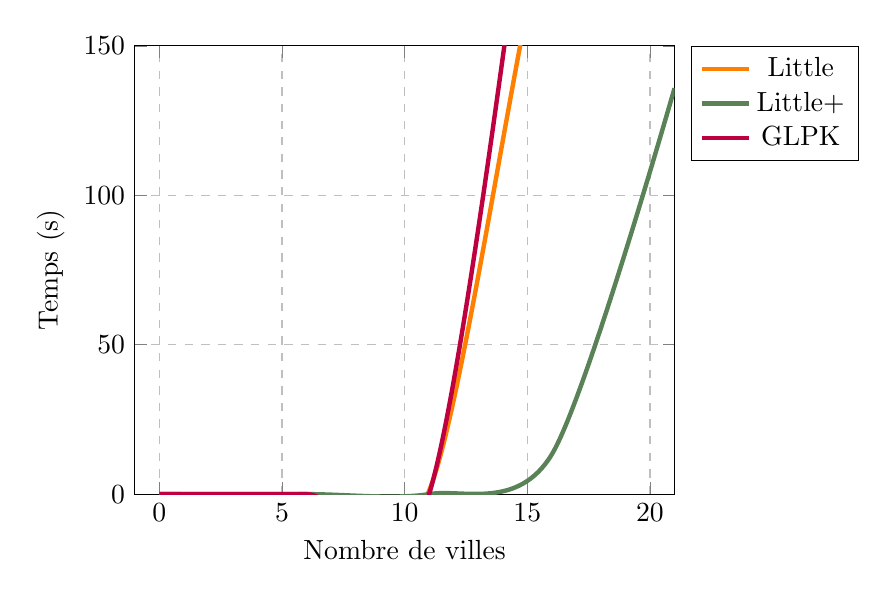
\begin{tikzpicture}
\begin{axis}
[
    xlabel={Nombre de villes},
    ylabel={Temps (s)},
    legend pos=outer north east,
    ymajorgrids=true,
    xmajorgrids=true,
    grid style=dashed,
    unbounded coords=jump,
    xmin=-1, xmax=21,
    ymin=0, ymax=150
]
\addplot [orange, ultra thick] plot [smooth] coordinates {(0,0) (6,0.000386) (11, 1.226015) (16, 200) (21, 300)};
\addplot [greenish, ultra thick] plot [smooth] coordinates {(0,0) (6,0.000167) (11, 0.005285) (16, 13.312551) (21, 135.795077)};
\addplot [purple, ultra thick] plot [smooth] coordinates {(0,0) (6,0) (11, 0.1) (16, 268.2) (21, 600)};
\legend{Little, Little+, GLPK}
\end{axis}
\end{tikzpicture}

\end{center}

\textbf{Au-delà de 20 villes, le temps de calcul devient prohibitive pour les 3 implémentations par sa nature exponentielle.}

Little+ possède la meilleure implémentation, en retirant les sous-tours, on économise des itérations et du temps de recherche.

\end{document}